\documentclass[10pt,a4paper]{article}
\usepackage[utf8]{inputenc}
\usepackage{amsmath}
\usepackage{amsfonts}
\usepackage{amssymb}
\usepackage{amsthm}
\usepackage{polynom} % Polynomdivision
\usepackage{url,xspace,boxedminipage}   % Accurate display of URLs
\usepackage{csquotes} % Quotes
\usepackage{pdfpages} % include whole PDF pages



\title{\textbf{\huge Grundlagen der Wissensverarbeitung
\\\Large Blatt 2}}
\author{Daniel Speck, Lena Niermeyer}
\date{23.10.2015}

\setlength{\topmargin}{-1.0cm}
\setlength{\textheight}{650pt}


\begin{document}


	% Titel, Autor & Abgabedatum
	\maketitle


			
	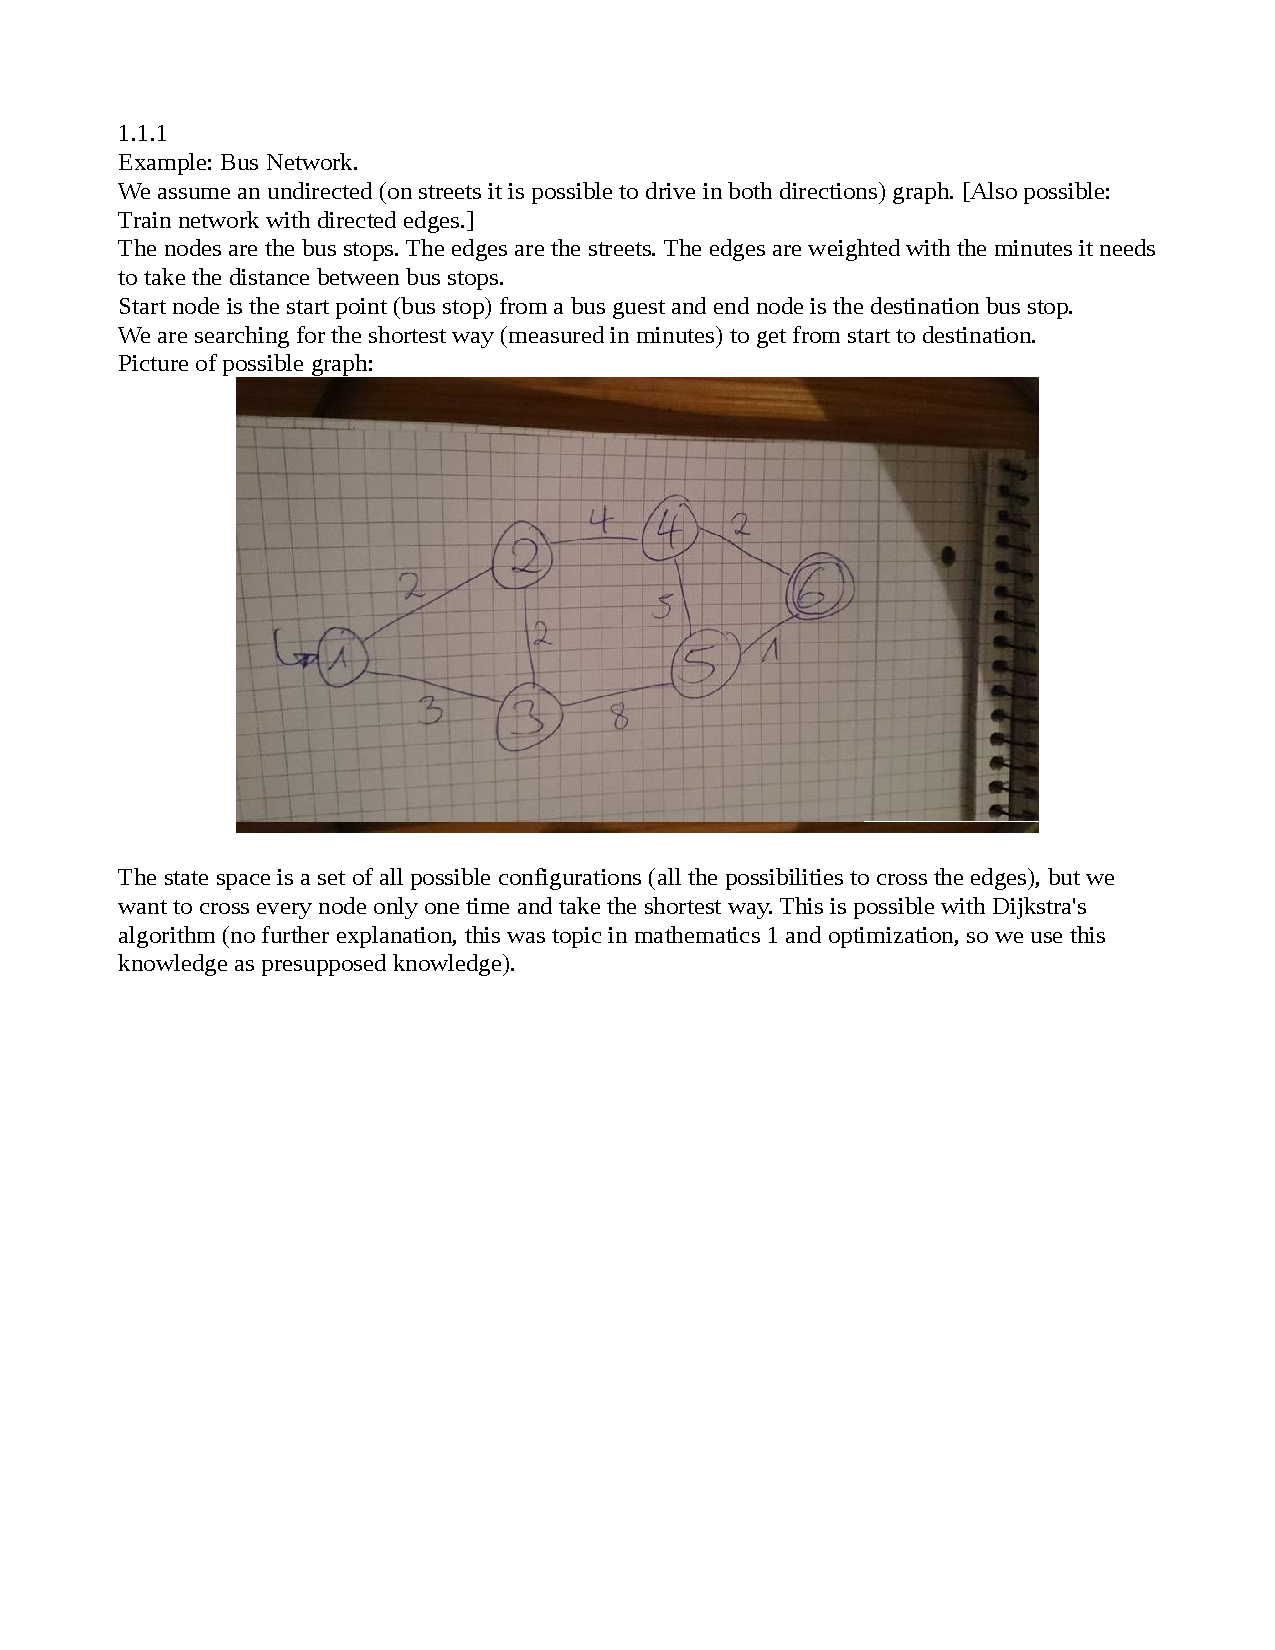
\includepdf{211.pdf}
	
	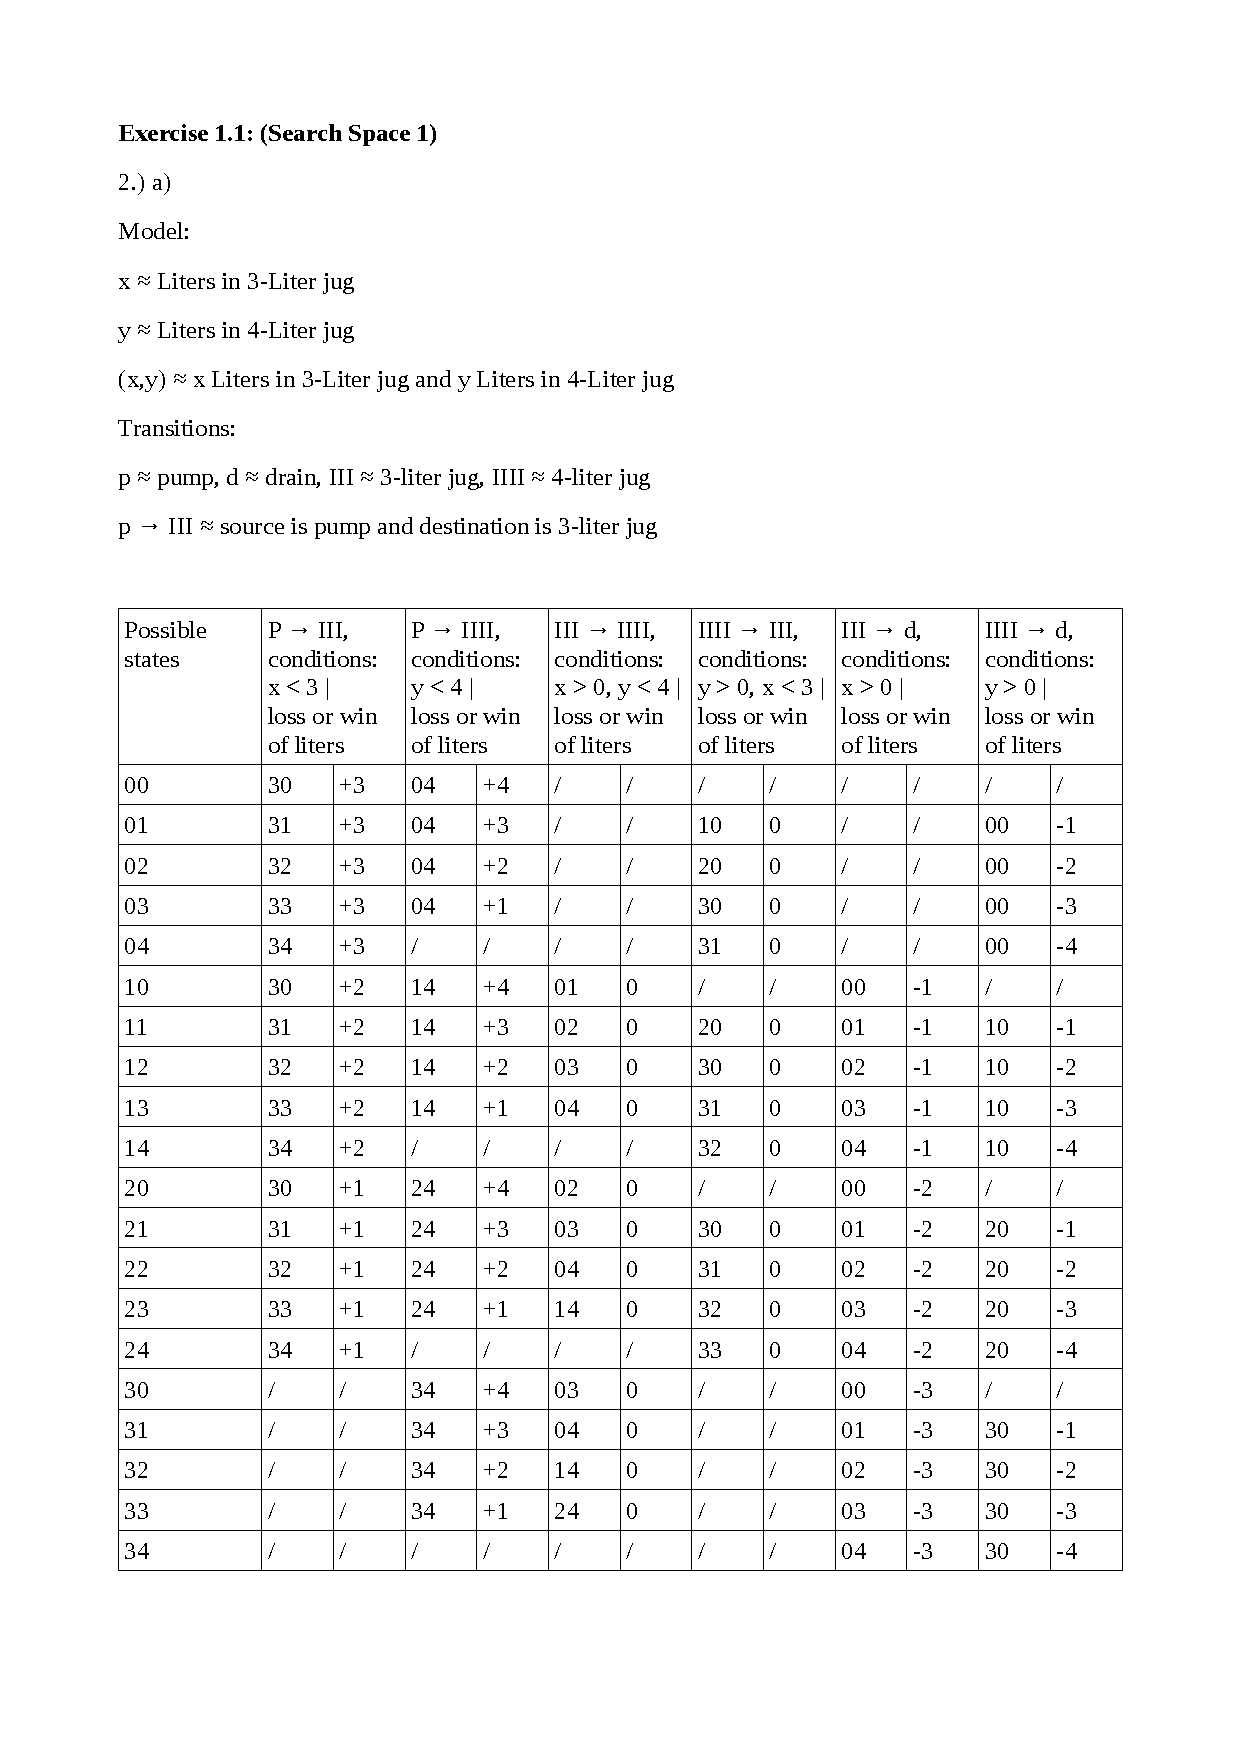
\includepdf[pages={1-3}]{212.pdf}
	
	
	\section*{Aufgabe 2.2 (Search Space 2)}

		In our last assignment one given example for AI scenarios was \enquote{navigating through a labyrinth}. Mazes/Labyrinths could be found in many computer games and most path finding solutions for AIs in such games could solved via searching.
		\\
		\textit{Pacman}, a classic computer game, was one of our examples for computer games with mazes. The player has to navigate Pacman through the maze and collect points represented by little dots. Considering the very basic version of Pacman the play area has about 150 fields, each field has one point by default and the point can be collected by Pacman. Additionally there are 4 ghosts chasing Pacman.
		\\
		For a solution utilizing searching this game could be modeled by a graph. Each node would represent one of 6 possible booleans:
		
		\begin{itemize}
			\item boolean1: point is present (not yet collected) or point is already collected by Pacman
			\item boolean2: Pacman is at this location or not
			\item boolean3 to 6: Ghost1, \dots, Ghost4 is at this location or not
		\end{itemize}
		
		\noindent 150 locations with 6 booleans each results in $150^6 = 11,390,625,000,000 \approx 1.139*10^{13}$ nodes for representing every possible state in the game. The edges would be the transitions between the states, so basically the movements of Pacman and the Ghosts as well as the action of collecting a point. There would be only one start state and therefore only one start node in the graph in the very basic version of Pacman, because in this version Pacman always starts at the same location: some points downwards from the center. The ghosts always start in the center.
		\\
		The graph has multiple end states, because every node where the \enquote{Pacman boolean} is true (so Pacman is present at this state/node) and the at least one of the \enquote{Ghost booleans} is true, the game ends by reason of Pacman has been eaten by the Ghosts and therefore the game is lost.
		\\
		Furthermore every node where all \enquote{point is present}-booleans are false (so Pacman has collected all available points) is an end state, because Pacman has won the game.
		
		

\end{document}





